

\tikzset{every picture/.style={line width=0.75pt}} %set default line width to 0.75pt        

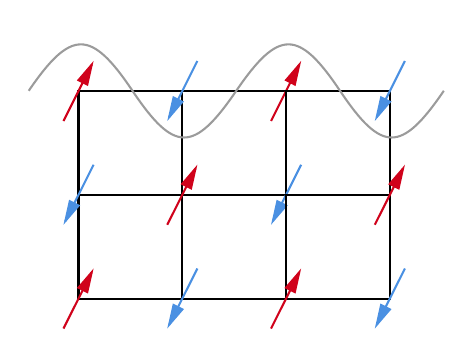
\begin{tikzpicture}[x=0.75pt,y=0.75pt,yscale=-1,xscale=1]
%uncomment if require: \path (0,300); %set diagram left start at 0, and has height of 300

%Shape: Square [id:dp7968380272014384] 
\draw   (148,62) -- (198,62) -- (198,112) -- (148,112) -- cycle ;
%Shape: Square [id:dp08936498453558128] 
\draw   (98,62) -- (148,62) -- (148,112) -- (98,112) -- cycle ;
%Shape: Square [id:dp6338164799723338] 
\draw   (98,112) -- (148,112) -- (148,162) -- (98,162) -- cycle ;
%Shape: Square [id:dp5647790600566112] 
\draw   (148,112) -- (198,112) -- (198,162) -- (148,162) -- cycle ;
%Straight Lines [id:da4505706138663077] 
\draw [color={rgb, 255:red, 208; green, 2; blue, 27 }  ,draw opacity=1 ]   (90.75,76.46) -- (104.35,49.33) ;
\draw [shift={(105.25,47.54)}, rotate = 476.63] [fill={rgb, 255:red, 208; green, 2; blue, 27 }  ,fill opacity=1 ][line width=0.08]  [draw opacity=0] (12,-3) -- (0,0) -- (12,3) -- cycle    ;
%Straight Lines [id:da8302639980131186] 
\draw [color={rgb, 255:red, 74; green, 144; blue, 226 }  ,draw opacity=1 ]   (155.25,47.54) -- (141.65,74.67) ;
\draw [shift={(140.75,76.46)}, rotate = 296.63] [fill={rgb, 255:red, 74; green, 144; blue, 226 }  ,fill opacity=1 ][line width=0.08]  [draw opacity=0] (12,-3) -- (0,0) -- (12,3) -- cycle    ;
%Straight Lines [id:da07392319534895608] 
\draw [color={rgb, 255:red, 208; green, 2; blue, 27 }  ,draw opacity=1 ]   (140.75,126.46) -- (154.35,99.33) ;
\draw [shift={(155.25,97.54)}, rotate = 476.63] [fill={rgb, 255:red, 208; green, 2; blue, 27 }  ,fill opacity=1 ][line width=0.08]  [draw opacity=0] (12,-3) -- (0,0) -- (12,3) -- cycle    ;
%Straight Lines [id:da29949826504712806] 
\draw [color={rgb, 255:red, 208; green, 2; blue, 27 }  ,draw opacity=1 ]   (90.75,176.46) -- (104.35,149.33) ;
\draw [shift={(105.25,147.54)}, rotate = 476.63] [fill={rgb, 255:red, 208; green, 2; blue, 27 }  ,fill opacity=1 ][line width=0.08]  [draw opacity=0] (12,-3) -- (0,0) -- (12,3) -- cycle    ;
%Straight Lines [id:da10136846066630589] 
\draw [color={rgb, 255:red, 208; green, 2; blue, 27 }  ,draw opacity=1 ]   (190.75,76.46) -- (204.35,49.33) ;
\draw [shift={(205.25,47.54)}, rotate = 476.63] [fill={rgb, 255:red, 208; green, 2; blue, 27 }  ,fill opacity=1 ][line width=0.08]  [draw opacity=0] (12,-3) -- (0,0) -- (12,3) -- cycle    ;
%Straight Lines [id:da18679469569417329] 
\draw [color={rgb, 255:red, 74; green, 144; blue, 226 }  ,draw opacity=1 ]   (105.25,97.54) -- (91.65,124.67) ;
\draw [shift={(90.75,126.46)}, rotate = 296.63] [fill={rgb, 255:red, 74; green, 144; blue, 226 }  ,fill opacity=1 ][line width=0.08]  [draw opacity=0] (12,-3) -- (0,0) -- (12,3) -- cycle    ;
%Straight Lines [id:da9509291375625459] 
\draw [color={rgb, 255:red, 74; green, 144; blue, 226 }  ,draw opacity=1 ]   (155.25,147.54) -- (141.65,174.67) ;
\draw [shift={(140.75,176.46)}, rotate = 296.63] [fill={rgb, 255:red, 74; green, 144; blue, 226 }  ,fill opacity=1 ][line width=0.08]  [draw opacity=0] (12,-3) -- (0,0) -- (12,3) -- cycle    ;
%Shape: Square [id:dp7989800051587621] 
\draw   (198,62) -- (248,62) -- (248,112) -- (198,112) -- cycle ;
%Straight Lines [id:da025654938728039145] 
\draw [color={rgb, 255:red, 74; green, 144; blue, 226 }  ,draw opacity=1 ]   (205.25,97.54) -- (191.65,124.67) ;
\draw [shift={(190.75,126.46)}, rotate = 296.63] [fill={rgb, 255:red, 74; green, 144; blue, 226 }  ,fill opacity=1 ][line width=0.08]  [draw opacity=0] (12,-3) -- (0,0) -- (12,3) -- cycle    ;
%Shape: Square [id:dp21923612897643863] 
\draw   (198,112) -- (248,112) -- (248,162) -- (198,162) -- cycle ;
%Straight Lines [id:da2934635233522882] 
\draw [color={rgb, 255:red, 208; green, 2; blue, 27 }  ,draw opacity=1 ]   (190.75,176.46) -- (204.35,149.33) ;
\draw [shift={(205.25,147.54)}, rotate = 476.63] [fill={rgb, 255:red, 208; green, 2; blue, 27 }  ,fill opacity=1 ][line width=0.08]  [draw opacity=0] (12,-3) -- (0,0) -- (12,3) -- cycle    ;
%Straight Lines [id:da9412499087817388] 
\draw [color={rgb, 255:red, 74; green, 144; blue, 226 }  ,draw opacity=1 ]   (255.25,47.54) -- (241.65,74.67) ;
\draw [shift={(240.75,76.46)}, rotate = 296.63] [fill={rgb, 255:red, 74; green, 144; blue, 226 }  ,fill opacity=1 ][line width=0.08]  [draw opacity=0] (12,-3) -- (0,0) -- (12,3) -- cycle    ;
%Straight Lines [id:da18617934942542336] 
\draw [color={rgb, 255:red, 74; green, 144; blue, 226 }  ,draw opacity=1 ]   (255.25,147.54) -- (241.65,174.67) ;
\draw [shift={(240.75,176.46)}, rotate = 296.63] [fill={rgb, 255:red, 74; green, 144; blue, 226 }  ,fill opacity=1 ][line width=0.08]  [draw opacity=0] (12,-3) -- (0,0) -- (12,3) -- cycle    ;
%Straight Lines [id:da24257455825409324] 
\draw [color={rgb, 255:red, 208; green, 2; blue, 27 }  ,draw opacity=1 ]   (240.75,126.46) -- (254.35,99.33) ;
\draw [shift={(255.25,97.54)}, rotate = 476.63] [fill={rgb, 255:red, 208; green, 2; blue, 27 }  ,fill opacity=1 ][line width=0.08]  [draw opacity=0] (12,-3) -- (0,0) -- (12,3) -- cycle    ;
%Shape: Sine Wave Form [id:dp4769190459095818] 
\draw  [color={rgb, 255:red, 155; green, 155; blue, 155 }  ,draw opacity=1 ] (74,61.91) .. controls (94.35,32.16) and (103.94,32) .. (123.99,61.91) .. controls (144.06,91.82) and (153.47,92) .. (174,61.91) ;
%Shape: Sine Wave Form [id:dp8043046043167636] 
\draw  [color={rgb, 255:red, 155; green, 155; blue, 155 }  ,draw opacity=1 ] (174,61.91) .. controls (194.35,32.16) and (203.94,32) .. (223.99,61.91) .. controls (244.06,91.82) and (253.47,92) .. (274,61.91) ;




\end{tikzpicture}